%Version 1.0 May 2025
%%%%%%%%%%%%%%%%%%%%%%%%%%%%%%%%%%%%%%%%%%%%%%%%%%%%%%%%%%%%%%%%%%%%%%
%%                                                                 %%
%% Please do not use \input{...} to include other tex files.       %%
%% Submit your LaTeX manuscript as one .tex document.              %%
%%                                                                 %%
%% All additional figures and files should be attached             %%
%% separately and not embedded in the \TeX\ document itself.       %%
%%                                                                 %%
%%%%%%%%%%%%%%%%%%%%%%%%%%%%%%%%%%%%%%%%%%%%%%%%%%%%%%%%%%%%%%%%%%%%%

%%\documentclass[referee,sn-basic]{sn-jnl}% referee option is meant for double line spacing

%%=======================================================%%
%% to print line numbers in the margin use lineno option %%
%%=======================================================%

%%=========================================================================================%%
%% the documentclass is set to pdflatex as default. You can delete it if not appropriate.  %%
%%=========================================================================================%%

%%\documentclass[sn-basic]{sn-jnl}% Basic Springer Nature Reference Style/Chemistry Reference Style

%%Note: the following reference styles support Namedate and Numbered referencing. By default the style follows the most common style. To switch between the options you can add or remove “Numbered” in the optional parenthesis. 
%%The option is available for: sn-basic.bst, sn-chicago.bst%  
 
%%\documentclass[pdflatex,sn-nature]{sn-jnl}% Style for submissions to Nature Portfolio journals
%%\documentclass[pdflatex,sn-basic]{sn-jnl}% Basic Springer Nature Reference Style/Chemistry Reference Style
\documentclass[pdflatex,sn-mathphys-num]{sn-jnl}% Math and Physical Sciences Numbered Reference Style
%%\documentclass[pdflatex,sn-mathphys-ay]{sn-jnl}% Math and Physical Sciences Author Year Reference Style
%%\documentclass[pdflatex,sn-aps]{sn-jnl}% American Physical Society (APS) Reference Style
%%\documentclass[pdflatex,sn-vancouver-num]{sn-jnl}% Vancouver Numbered Reference Style
%%\documentclass[pdflatex,sn-vancouver-ay]{sn-jnl}% Vancouver Author Year Reference Style
%%\documentclass[pdflatex,sn-apa]{sn-jnl}% APA Reference Style
%%\documentclass[pdflatex,sn-chicago]{sn-jnl}% Chicago-based Humanities Reference Style

%%%% Standard Packages
%%<additional latex packages if required can be included here>

\usepackage{tikz}
\usetikzlibrary{shapes.geometric, arrows, positioning, fit, backgrounds}
\usepackage{graphicx}%
\usepackage{multirow}%
\usepackage{amsmath,amssymb,amsfonts}%
\usepackage{amsthm}%
\usepackage{mathrsfs}%
\usepackage[title]{appendix}%
\usepackage{xcolor}%
\usepackage{textcomp}%
\usepackage{manyfoot}%
\usepackage{booktabs}%
\usepackage{algorithm}%
\usepackage{algorithmicx}%
\usepackage{algpseudocode}%
\usepackage{listings}%


%% as per the requirement new theorem styles can be included as shown below
\theoremstyle{thmstyleone}%
\newtheorem{theorem}{Theorem}%  meant for continuous numbers
%%\newtheorem{theorem}{Theorem}[section]% meant for sectionwise numbers
%% optional argument [theorem] produces theorem numbering sequence instead of independent numbers for Proposition
\newtheorem{proposition}[theorem]{Proposition}% 
%%\newtheorem{proposition}{Proposition}% to get separate numbers for theorem and proposition etc.

\theoremstyle{thmstyletwo}%
\newtheorem{example}{Example}%
\newtheorem{remark}{Remark}%

\theoremstyle{thmstylethree}%
\newtheorem{definition}{Definition}%

\raggedbottom
% \unnumbered% uncomment this for unnumbered level heads

\begin{document}

\title[Article Title]{Comparative Evaluation of the Red Deer Algorithm for Load Balancing in Cloud Computing
}

%%=============================================================%%
%% GivenName	-> \fnm{Joergen W.}
%% Particle	-> \spfx{van der} -> surname prefix
%% FamilyName	-> \sur{Ploeg}
%% Suffix	-> \sfx{IV}
%% \author*[1,2]{\fnm{Joergen W.} \spfx{van der} \sur{Ploeg} 
%%  \sfx{IV}}\email{iauthor@gmail.com}
%%=============================================================%%

\author[1]{\fnm{Krish} \sur{Sharma}}
\author[1]{\fnm{Tanmay} \sur{Tushar}}
\author*[1]{\fnm{Nripendranarayan} \sur{Das} \email{nripendranarayan.das@jaipur.manipal.edu}}
\author*[2]{\fnm{Ashish} \sur{Jain} \email{ashishjn.research@gmail.com}}


\affil[1]{\orgdiv{Department of Information Technology}, \orgname{Manipal University Jaipur}, \orgaddress{\city{Jaipur}, \postcode{303007}, \state{Rajasthan}, \country{India}}}

\affil[2]{\orgdiv{Department Name}, \orgname{College Name}, \orgaddress{\city{Jaipur}, \state{Rajasthan}, \country{India}}}

\abstract{This paper investigates the critical challenge of load balancing in cloud computing, a key factor influencing the performance, reliability, and efficiency of cloud based services. With the rise of cloud computing technologies, the need for effective workload distribution across heterogeneous and geographically distributed resources has become increasingly complex. Load balancing is categorized as an NP-hard problem due to its vast solution space, necessitating the use of metaheuristic algorithms for efficient problem solving. In this study, we propose a load balancing approach based on Red Deer Algorithm (RDA). Additionally, a comparative performance analysis is conducted between various metaheuristic load balancing algorithms to evaluate their effectiveness based on metrics such as makespan time, response time, resource utilization. Simulation results using CloudSim demonstrate that the RDA based method significantly reduces costs and response time. The findings support the potential of metaheuristic techniques to provide near optimal solutions within reasonable timeframes, thereby enhancing Quality of Service (QoS) and resource utilization in cloud environments.}


\keywords{Metaheuristic Algorithms, Red Deer Algorithm, Cloud Computing, Grey Wolf Optimization, Genetic Algorithm}

\maketitle
\clearpage

\section{Introduction}\label{sec1}
Cloud computing is a model for delivering resources such as servers, storage systems, databases, networking facilities, software applications, and analytics tools over the Internet, commonly referred to as “the cloud” \cite{cloudComputing}. The adoption of cloud computing enables users to access applications from anywhere in the world. This approach differs significantly from traditional hosting models due to two key entities: the Cloud Service Provider (CSP) and the Cloud Service User (CSU) \cite{bib2}. In most cases, the use of cloud services involves associated costs.

Cloud computing services typically follow a “pay-as-you-go” and “on-demand” model, allowing customers to avoid long-term contractual commitments. The self-service capability enables users to provision resources automatically without requiring manual intervention, sales processes, or complex service setup procedures. This automation simplifies service acquisition and enhances usability while contributing to competitive pricing \cite{cloudComputing2}.

Due to the dynamic and distributed nature of cloud computing environments, where resources are provisioned and consumed over the Internet as needed, effective resource management is essential. As the number of applications and users that rely on cloud services continues to grow, it becomes increasingly important to ensure that workloads are efficiently distributed across available computing nodes. This distribution helps maintain system responsiveness, reliability, and overall performance. Load balancing plays a critical role in achieving this objective \cite{bib3}.

Load balancing refers to the efficient and equitable distribution of tasks across computing resources, such as virtual machines (VMs), to maintain optimal resource utilization and meet system performance requirements (e.g. processor load, primary and secondary memory usage, latency and network load) \cite{loadBalancing}. When certain VMs experience higher workloads than others, overall system efficiency decreases. Load balancing addresses this issue by allowing intelligent distribution of tasks among available computing resources \cite{bib6}.

The primary objective of load balancing is to maintain acceptable levels of resource utilization measured in terms of CPU usage, memory consumption, response time, and network traffic while satisfying user requirements and maximizing resource efficiency \cite{loadBalancing3}. An effective load balancing mechanism considers both the current state of resource availability and the specific requirements of the incoming tasks to make informed allocation decisions. This approach helps reduce traffic bottlenecks, improve system performance, increase throughput, and ensure optimal utilization of cloud infrastructure.

Therefore, the choice of load balancing strategy is of critical importance \cite{loadBalancing2}. Traditional deterministic or rule-based algorithms often struggle to handle the scale, complexity, and dynamic nature of cloud environments. In contrast, metaheuristic algorithms have emerged as promising solutions for load balancing problems, as they can efficiently explore large solution spaces and identify near optimal solutions within reasonable computational time \cite{bib5}.

A metaheuristic solution can be defined as an interactive set of processes that govern the exploration and exploitation of the search landscape \cite{bib4, Blum2003}. Metaheuristic methods are one of the strategies that can be applied to resolve performance issues, for example, task scheduling \cite{bib7, Li2018}. Metaheuristic algorithms are high-level problem-independent methods that guide lower level heuristics to finding optimal or near-optimal solutions to complicated optimization problems. These algorithms, e.g., Genetic Algorithms (GA), Particle Swarm Optimization (PSO) \cite{Kennedy1995}, and Ant Colony Optimization (ACO) \cite{Dorigo1992}, are inspired by natural phenomena like evolutionary processes, collective behavior, or reproduction strategies of certain animal species \cite{bib4, Yang2010}. Even though they do not guarantee the achievement of a global optimum, such approaches are well adapted to providing acceptable solutions for NP-hard problems, especially if exhaustive search is computationally infeasible. Their flexibility, scalability, and adaptability make them particularly well adapted to dynamic environments like cloud computing, where conditions change constantly and optimum task-resource assignment needs constant re-tuning \cite{Buyya2010}.

\begin{figure}[htbp]
  \centering
  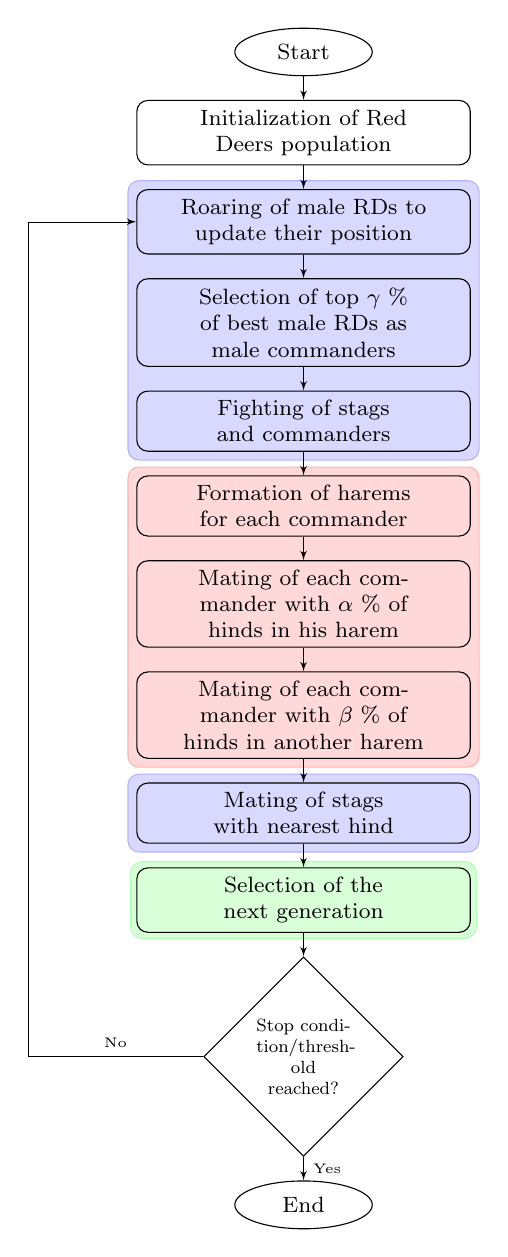
\begin{tikzpicture}[
      node distance = 0.5cm,
      auto,
      block/.style={rectangle, draw, rounded corners, text width=4cm, text centered, minimum height=0.6cm, font=\footnotesize},
      ellipse_block/.style={ellipse, draw, text width=1cm, text centered, minimum height=0.6cm, font=\footnotesize},
      decision/.style={diamond, draw, text width=1.5cm, text centered, minimum height=0.6cm, font=\footnotesize},
      line/.style={draw, -latex', very thin},
      blue_block/.style={block, fill=blue!15},
      red_block/.style={block, fill=red!15},
      green_block/.style={block, fill=green!15}
  ]
  
  
  \node [ellipse_block] (start) {Start};
  \node [block, below=0.3cm of start] (init) {Initialization of Red Deers population};
  \node [blue_block, below=0.3cm of init] (roar) {Roaring of male RDs to update their position};
  \node [blue_block, below=0.3cm of roar] (select) {Selection of top $\gamma$ \% of best male RDs as male commanders};
  \node [blue_block, below=0.3cm of select] (fight) {Fighting of stags and commanders};
  \node [red_block, below=0.3cm of fight] (harem) {Formation of harems for each commander};
  \node [red_block, below=0.3cm of harem] (mate1) {Mating of each commander with $\alpha$ \% of hinds in his harem};
  \node [red_block, below=0.3cm of mate1] (mate2) {Mating of each commander with $\beta$ \% of hinds in another harem};
  \node [blue_block, below=0.3cm of mate2] (mate3) {Mating of stags with nearest hind};
  \node [green_block, below=0.3cm of mate3] (next) {Selection of the next generation};
  \node [decision, below=0.3cm of next, scale=0.8] (stop) {Stop condition/threshold reached?};
  \node [ellipse_block, below=0.3cm of stop] (end) {End};
  

  \path [line] (start) -- (init);
  \path [line] (init) -- (roar);
  \path [line] (roar) -- (select);
  \path [line] (select) -- (fight);
  \path [line] (fight) -- (harem);
  \path [line] (harem) -- (mate1);
  \path [line] (mate1) -- (mate2);
  \path [line] (mate2) -- (mate3);
  \path [line] (mate3) -- (next);
  \path [line] (next) -- (stop);
  \path [line] (stop) -- node[right, font=\tiny] {Yes} (end);
  \path [line] (stop) -| node[near start, above, font=\tiny] {No} ++(-3.5,0) |- (roar);
  

  \begin{scope}[on background layer]
    \node[fit=(roar)(select)(fight), fill=blue!15, rounded corners, draw=blue!30, inner sep=3pt] {};
    \node[fit=(harem)(mate1)(mate2), fill=red!15, rounded corners, draw=red!30, inner sep=3pt] {};
    \node[fit=(mate3), fill=blue!15, rounded corners, draw=blue!30, inner sep=3pt] {};
    \node[fit=(next), fill=green!15, rounded corners, draw=green!30, inner sep=2pt] {};
  \end{scope}
  
  \end{tikzpicture}
  \caption{Flow Chart of RDA \cite{red_deer}}
  \label{fig:rda-flowchart}
\end{figure}


Currently, the selection of the most suitable cloud services is optimized using QoS criteria, which helps address challenges related to connectivity and the definition of QoS parameters \cite{QoS}. QoS remains one of the most critical aspects in addressing challenges within cloud computing. In the present study, a novel load balancing technique is introduced based on the RDA, integrated with QoS considerations to identify the best possible solution. RDA draws inspiration from the natural mating behavior of red deer \cite{red_deer}. The algorithm begins by initializing a population of red deer, which are then classified into male and female individuals. All male red deer update their positions and then mate. After all mating operations, a new generation is formed by selecting offspring based on fitness, and the process iterates until a predefined number of generations is reached \cite{red_deer}. This biologically inspired structure allows RDA to effectively balance exploration and exploitation, making it highly suitable for solving complex optimization problems such as load balancing in cloud computing, where dynamic resource allocation and efficiency are essential \cite{red_deer_Pradhan2022}.

The structure of rest of this paper follows as: Section \ref{sec2} discusses related work in the domain. Section \ref{sec3} presents the proposed model. The development of the RDA in accordance with the proposed model is detailed in Section \ref{sec4}. Section \ref{sec5} outlines the experimental setup, while Section \ref{sec6} presents the results and analysis. Finally, Section \ref{sec7} concludes the paper with future research directions.


\section{Related Work}\label{sec2}


Goyal and Singh \cite{bib10} proposed the Ant-based Load Balancing Algorithm (ALBA) for dynamic load balancing in grid computing environments. Unlike traditional ACO, in which pheromone trails are deposited on paths between nodes, ALBA associates pheromone directly with resources to indicate their current load levels. When a task completes successfully on a resource, its pheromone value is increased to signal light load, whereas task failure triggers a pheromone decrease to signal heavy load. Task assignment is then guided by transition probabilities computed from these pheromone values, directing incoming tasks toward the least loaded resources. The algorithm was evaluated using GridSim across two scenarios: varying the number of tasks from 25 to 100 with a fixed resource pool of 10, and varying the number of resources from 10 to 30 with a fixed task count of 75. Results demonstrated that ALBA achieved significantly more uniform resource utilization compared to the baseline without load balancing (WALBA), with a standard deviation of load distribution not exceeding 0.77, compared to a range of 2.35 to 3.18 for WALBA.
However, several critical limitations substantially restrict the practical applicability of this work. First, and most fundamentally, ALBA is designed and evaluated exclusively for grid computing, not cloud computing. The architectural assumptions of the paper, including geographically distributed independent resources and static resource pools, differ significantly from the VM-based, virtualized, and elastically scalable nature of cloud environments, making direct applicability to cloud load balancing questionable. Second, the comparative evaluation is conducted solely against WALBA, a trivial baseline that performs no load balancing whatsoever. The absence of comparison against other established metaheuristic approaches such as PSO, GA, or other ACO variants makes it impossible to objectively position ALBA's performance within the broader literature. Third, the evaluation is limited to a maximum of 100 tasks and 30 resources, which represents a very small scale relative to real-world grid or cloud deployments, raising serious concerns about scalability. Fourth, the study does not evaluate critical QoS metrics such as makespan, task response time, energy consumption, or fault tolerance, reporting only resource utilization and standard deviation of load distribution. This narrow evaluation scope makes it difficult to assess the algorithm's overall effectiveness as a scheduling solution.

Kruekaew and Kimpan \cite{bib12} proposed the Heuristic Task Scheduling with Artificial Bee Colony (HABC) algorithm, which combines swarm intelligence from the ABC algorithm with heuristic scheduling strategies, namely First Come First Serve (FCFS), Smallest Job First (SJF), and Largest Job First (LJF), to optimize VM scheduling and load distribution in cloud computing environments. The proposed method was evaluated against ACO, PSO, and IPSO using the CloudSim simulation toolkit across twelve datasets spanning four distribution types: random, normal, right-skewed, and left-skewed. Experimental results demonstrated that HABC with the LJF heuristic consistently achieved the lowest minimum, maximum, and average makespan values, as well as the lowest degree of load imbalance, across both homogeneous and heterogeneous environments. Notably, the standard deviation of VM processing times under HABC was substantially lower than that of ACO, PSO, and IPSO, indicating a more balanced workload distribution. However, several critical limitations warrant attention. First, the evaluation was conducted exclusively in a simulated environment using CloudSim, and the authors themselves acknowledged that experiments were performed on a limited number of datasets, with plans to extend to larger, real-world workloads in future work. This raises concerns about the generalizability of the results to dynamic, production-scale cloud deployments. Second, the study does not address task dependencies or priority-based scheduling beyond job length, which are common requirements in practical cloud workflows. Third, while HABC demonstrates strong makespan and load balancing performance, the study does not evaluate critical QoS parameters such as resource reliability, fault tolerance, energy consumption, or cost efficiency, which are essential metrics for comprehensive cloud scheduler assessment. Finally, the algorithm's performance is highly sensitive to parameter configuration, particularly the number of scout, employed, and onlooker bees, and the study does not propose an adaptive tuning mechanism, limiting its robustness across varying workload characteristics.



\begin{table}[h]
\caption{Comparison of related load balancing algorithms in cloud computing}\label{tab:relatedwork}
\begin{tabular*}{\textwidth}{@{\extracolsep\fill}p{2.5cm}p{2cm}p{3cm}p{3cm}}
\toprule
\textbf{Author(s)} & \textbf{Algorithm} & \textbf{Advantages} & \textbf{Limitations} 
\\
\midrule
Goyal and Singh \cite{bib10} & ALBA & More uniform resource utilization in grid environments & Grid-specific, only compared against a no-load-balancing baseline
\\
\\
Kruekaew and Kimpan \cite{bib12} & HABC, ABC & Minimizes makespan; improves load balance & Needs parameter tuning; high operational cost 
\\
\\
Sefati et al. \cite{bib9} & GWO & Lower response time and cost; considers reliability & Computational overhead; lacks security/scalability
\\
\\
Anbarkhan and Rakrouki \cite{Anbarkhan2023AnEP} & EPSO & Reduces particle dimensionality via workflow task preprocessing, improved initialization ensures higher initial solution quality, achieves lower makespan and cost compared to PSO and HPSO & Limited to small-scale workloads (max 300 tasks), single-objective fitness function ignores load balancing, energy, and fault tolerance; narrow comparative evaluation against only two baselines 
\\
\\
Lilhore et al. \cite{lilhore2025} & Hybrid WWO-ACO & 
Reduced task scheduling time, lower energy consumption, 
improved resource utilization, and superior load balancing 
across homogeneous and heterogeneous cloud environments & 
High computational overhead, performance variability across 
different cloud infrastructures, limited simulation scale, 
assumes independent tasks with no dependencies or deadlines
\\
\botrule
\end{tabular*}
\end{table}



Sefati et al. \cite{bib9} proposed a QoS-aware load balancing method for cloud 
computing environments utilizing the Grey Wolf Optimization (GWO) algorithm, 
inspired by the social hierarchy and cooperative hunting behavior of grey wolves. 
The method operates through a structured multi-step process: first, a cluster head 
is selected based on the node with the highest number of neighboring VMs; the GWO 
algorithm then dispatches wolf agents to explore the search space, calculating a 
load threshold for each VM defined as $\psi = AL + \sigma$, where $AL$ represents 
the average load across all VMs in the data center and $\sigma$ is the standard 
deviation of VM loads. VMs exceeding this threshold are classified as overloaded 
and excluded from task assignment, while underloaded VMs are ranked using a fitness 
factor that combines QoS reliability scores with load balancing values. The alpha 
and beta wolves then guide the selection of the most suitable underloaded VM for 
task allocation. The reliability of each VM is quantified using an exponential 
decay model that accounts for failure rate and task weight, directly integrating 
resource dependability into the scheduling decision. The algorithm was evaluated 
using CloudSim across task loads ranging from 20 to 80 tasks and benchmarked 
against ABC, PSO, and GA. Results demonstrated that GWO achieved the lowest 
average makespan of 6.85, compared to 8.57 for PSO, 9.57 for ABC, and 11.41 for 
GA, while also achieving the lowest average response time of 5.18 seconds and the 
lowest average operational cost of 43.71, consistently outperforming all three 
competing algorithms across all evaluated metrics.

However, several critical limitations substantially constrain the practical 
applicability and generalizability of this work. First, the evaluation is conducted 
on an extremely limited scale, with a maximum of only 80 tasks and a single data 
center configuration comprising three hosts, which is far too small to draw 
meaningful conclusions about algorithm behavior in realistic cloud deployments 
that routinely handle thousands of concurrent tasks across multiple data centers. 
The authors themselves acknowledge this limitation, explicitly suggesting in their 
future work that more data centers and VMs should be incorporated to improve the 
proposed method. Second, the comparative evaluation is restricted to ABC, PSO, 
and GA, all of which are relatively dated metaheuristic baselines. The study does 
not benchmark GWO against more recent and competitive algorithms such as hybrid 
metaheuristics or other nature-inspired approaches that have demonstrated superior 
performance in cloud scheduling literature, which limits the strength of the 
performance claims. Third, while the incorporation of resource reliability into 
the scheduling decision is a notable contribution that distinguishes this work 
from purely performance-oriented approaches, the study does not evaluate fault 
tolerance, energy consumption, or scalability, which are critical QoS dimensions 
in production cloud environments. The authors acknowledge this gap directly, 
recommending that future work incorporate accessibility, security, and scalability 
alongside reliability. Fourth, the algorithm assumes that all tasks are 
independent, with no dependencies or priorities among them, which is a significant 
simplification that reduces its applicability to real-world cloud workloads where 
tasks frequently form dependency graphs. The authors explicitly identify dynamic 
load balancing for dependent tasks as a key future research direction. Fifth, the 
GWO parameter configuration, including a population size of 10 and a maximum of 
100 iterations, is fixed and relatively small, and the study does not provide a 
sensitivity analysis or adaptive tuning mechanism, raising concerns about 
robustness across varying workload characteristics and cloud configurations.

Anbarkhan and Rakrouki \cite{Anbarkhan2023AnEP} proposed an Enhanced Particle Swarm Optimization (EPSO) algorithm to address the limitations of the standard PSO algorithm in scheduling workflow tasks within cloud computing environments. The core methodology involves three principal enhancements to the classical PSO framework: a workflow task model preprocessing stage that classifies tasks as either computationally intensive or IO-intensive using a directed acyclic graph (DAG) representation and merges related subtasks into unified independent task units, thereby reducing particle dimensionality, an improved particle initialization strategy that normalizes both resource computing capabilities and task data volumes, deterministically assigning the top 25\% most data intensive tasks to the highest performing resources while randomly allocating the remaining 75\%, ensuring a balance between initial solution quality and search space diversity and a self-adaptive fitness function defined as the reciprocal of the makespan, which aligns the particle optimization direction with the objective of minimizing overall task completion time. The algorithm was evaluated using CloudSim with an HP ProLiant DL380 G9 server configuration across workloads ranging from 10 to 300 tasks, with each algorithm executed 20 times and average results reported. Benchmarked against the standard PSO and the heuristic based HPSO, the EPSO achieved a workflow task scheduling time of 255.145 seconds for 300 tasks, compared to 394.156 seconds for HPSO and 459.562 seconds for PSO, and a corresponding cost of \$401.5 versus \$459.8 for HPSO and \$558.3 for PSO. For independent task scheduling under the same workload, EPSO recorded 225.523 seconds against 254.246 seconds for HPSO and 327.789 seconds for PSO. Convergence analysis further demonstrated that the algorithm stabilizes after approximately 25 iterations for a 100 task workflow, reflecting the effectiveness of the dimensionality reduction strategy.
However, several limitations merit critical consideration. First, the experimental evaluation is confined to a single fixed physical node configuration and a maximum of 300 tasks, which does not adequately represent the scale or heterogeneity of real world cloud deployments where thousands of concurrent tasks and heterogeneous multi datacenter environments are commonplace. Second, the particle initialization heuristic, while improving initial solution quality, applies a fixed 25/75 split between deterministic and random assignment without any adaptive mechanism to adjust this ratio based on workload characteristics or resource availability, which may lead to suboptimal initialization under highly skewed or dynamic task distributions. Third, the adaptive function is defined solely as the reciprocal of the makespan, meaning the optimization objective is restricted to execution time minimization, important practical objectives such as load balancing, energy consumption, fault tolerance, and VM utilization are entirely absent from the fitness formulation, as the authors themselves acknowledge in their future work discussion. Fourth, while the workflow task model preprocessing introduces a meaningful reduction in problem complexity, the task merging strategy is based on a binary compute intensive versus IO-intensive classification determined by a single global threshold condition, which may oversimplify the heterogeneous dependency structures found in real scientific workflows such as those modeled by Pegasus or Montage, where tasks exhibit mixed resource demands across different pipeline stages. Fifth, the comparative evaluation is limited to two baselines  the standard PSO and the HPSO of and does not include comparisons against other contemporary metaheuristic approaches such as ACO based, GA based, or more recent hybrid methods, which significantly constrains the ability to assess the EPSO algorithm's relative competitiveness within the broader state of the art.




Lilhore et al. \cite{lilhore2025} proposed a hybrid multi-objective optimization algorithm that integrates Water Wave Optimization (WWO) and ACO to address load balancing and resource allocation challenges in cloud computing environments. The hybrid model leverages ACO's local search capabilities for task scheduling, wherein ants probabilistically select resources based on pheromone levels and heuristic information, while WWO's global exploration mechanism, modeled on wave propagation, refraction, and breaking phenomena, is employed for broader resource allocation optimization. The two algorithms operate sequentially, with ACO generating initial solutions that serve as the starting population for the WWO phase, and the best solutions from both phases are combined through a Pareto-dominance framework to simultaneously optimize four competing objectives: response time, resource consumption, operational cost, and energy consumption. The algorithm was evaluated using CloudSim Plus 6.2.2 across five experimental scenarios, with workloads ranging from 500 to 2500 tasks and VM configurations of 50 to 200, and benchmarked against GA, SMO, WWO, and ACO. Results demonstrated that WWO-ACO achieved an average task scheduling duration of 1107.8 seconds for 2000 tasks and 150 VMs, substantially outperforming ACO (1407.32 s), GA (7378.72 s), SMO (7578.32 s), and WWO (8587.7 s). Additionally, the algorithm reduced energy consumption to 335.0 kJ for 100 VMs and 2500 tasks, compared to 400.4 kJ for GA and 344.9 kJ for ACO, while achieving balance degree values ranging from 0.87 to 0.95 across 200 VM configurations, indicating consistently equitable workload distribution.
However, several limitations warrant critical consideration. First, the authors themselves acknowledge that the algorithm incurs significant computational overhead, with a time complexity of O((N\textsubscript{ants} × N\textsubscript{iter} × D) + (N\textsubscript{waves} × N\textsubscript{iter} × D)), which may become prohibitive in large-scale or highly dynamic cloud deployments where real-time scheduling decisions are required. Second, the paper acknowledges performance variability across different cloud infrastructures and workload distributions, with the authors noting that additional parameter tuning may be necessary for different deployment contexts, which limits the algorithm's out-of-the-box generalizability. Third, while the evaluation employs both synthetic workloads and a real-world HPC2N log trace, the simulation environment is confined to a fixed configuration of three data centers and ten hosts, which does not fully represent the scale and heterogeneity of production cloud deployments. Fourth, the study does not address task dependencies, deadlines, or priority constraints, assuming all tasks to be independent and free, which is a significant restriction given that real-world cloud workflows frequently involve complex inter-task relationships. Finally, while the paper compares the algorithm against GA, SMO, WWO, and ACO, it does not benchmark against other recent hybrid metaheuristics specifically designed for cloud load balancing, such as GWO based or PSO based hybrid approaches, which limits the comprehensiveness of the comparative evaluation.

\section{Proposed Model}\label{sec3}

In cloud computing, vast networks of data centers and users are spread globally. When numerous user requests flood the cloud simultaneously, efficient organization and service delivery are essential. The cloud must distribute workloads evenly across resources to ensure fairness. Load balancing remains a key challenge, requiring equal distribution of tasks to maintain user satisfaction. Various load-balancing algorithms exist for distributed, grid, and cloud systems \cite{bib4}. This study introduces a novel method for load balancing based on QoS to minimize response time and resource allocation costs. The proposed approach employs the RDA algorithm to achieve effective load balancing in a cloud environment.

\begin{figure}[h]
\centering
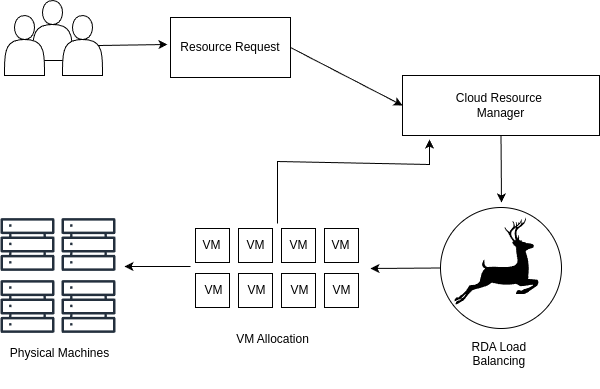
\includegraphics[width=0.9\textwidth]{Fig2.png}
\caption{The proposed load-balancing system}\label{LoadBalancing}
\end{figure}



\subsection{Problem Statement}\label{subsec3.1}

Consider cloud C, which consists of N physical machines, each containing M VMs.
\begin{equation}
C = \{PM_1, PM_2,\ldots,PM_N\}
\end{equation}

Additionally, every physical machine consists of multiple VMs configured as follows:
\begin{equation}
PM_i = \{VM_{i1}, VM_{i2},\ldots,VM_{iM}\}
\end{equation}

$VM_1$ represents the first virtual machine, and $VM_M$ denotes the final one. Our aim is to minimize costs and maximize the utilization of resources by evenly distributing workload across all the VMs. Efficient load balancing is the key to our approach; otherwise, the system would waste unnecessary time and energy on its tasks. To tackle this, our study proposes an efficient, multi-objective load-balancing approach using the RDA algorithm.

Our model treats the resource allocation as a multi-objective optimization problem and seeks to:
\begin{enumerate}
    \item Minimize the makespan time to enhance task completion time and efficiency,
    \item Maximize utilization of resources to improve infrastructure efficiency,
    \item Minimize costs to make it economically viable,
    \item Reduce response time to maintain QoS.
\end{enumerate}

These objectives tend to be conflicting with one another, and they need to be balanced properly. For example, aggressively reducing makespan may raise the demand for provisioning more resources, which can raise costs and lower overall utilization \cite{bib9}.

The model employs a weighted approach towards these objectives, allowing system administrators to assign weights to some measurements based on their intended use. This renders it adaptable to evolving requirements while maintaining the overall system performance.

\subsection{Parameters of QoS}\label{subsec3.2}

Makespan, utilization of resources, response time, and cost-effectiveness are performance measures that, collectively, constitute a holistic framework for quantifying the effectiveness of resource allocation policies \cite{bib12}. The model introduced here attempts to promote resource allocation in cloud environments by balancing these performance measures.

\subsubsection{Makespan}\label{subsubsec3.2.1}
Makespan time represents the total time required to complete the scheduled tasks \cite{bib9}. In our model, we are considering the maximum makespan time among all VMs, it is given as following:

\begin{equation} \label{eq3}
\text{Makespan} = \max\{CT_1, CT_2, \dots, CT_M\}
\end{equation}% Figure number displayed separately as in original

Where CT(i) represents the completion time of virtual machine i, and M is the total number of available VMs. Our goal is to reduce makespan time to guarantee timely execution of tasks.

\subsubsection{Resource Utilization}\label{subsubsec3.2.2}
Resource utilization is the ratio of time a VM is actively processing tasks to the makespan time \cite{bib9}. Resource utilization for an individual VM:

\begin{equation} \label{eq4}
\text{Utilization}_{VM_j} = \frac{\sum_{i=1}^{n} PT_{ij}}{\text{Makespan}}
\end{equation}

Where \( PT_{ij} \) represents the processing time of task i on \( VM_j \). The total resource utilization across the cloud is then determined by:

\begin{equation} \label{eq5}
\text{Resource Utilization} = \frac{\sum_{j=1}^{m} \text{Utilization}_{VM_j}}{m}
\end{equation}

This metric provides information on how effectively available computational resources are being used in the present situation. Increased utilization ratios indicate better resource management, which can reduce the operational expenses as well as the environmental impact.

% \subsubsection{Response Time}\label{subsubsec3.2.3}

% Response time is a critical service quality indicator that measures a system's ability to process requests promptly\cite{bib9}. We evaluate response time using the response-to-request ratio:

% \begin{equation}
% RA_{RR} = \frac{RES_k}{REC_k}
% \end{equation}

% where \( RES_k \) represents the work redistributed by resource \( k \) within a specific timeframe (measured in milliseconds), and \( REC_k \) denotes the number of collected requests. This ratio provides insight into the system's responsiveness under various load conditions.

\subsubsection{Response Time (RT)}\label{subsubsec3.2.3}

 We model the response time in our model by utilizing SpaceShared basis queuing behavior of tasks on Vms. SpaceShared is a resource allocation policy where each cloudlet uses a single core at a time, and the remaining wait in a queue until other resources become available to be utilized \cite{space-shared}.

The response time is defined as the time that a cloudlet takes from the time of arrival to its completion time. In our model, we leveraged the SpaceShared model to simulate the queuing behavior of tasks on Vms. The SpaceShared model of allocation is a resource allocation policy where each cloudlet can get only a single core at a time, while others must wait in a queue until other resources become available \cite{space-shared}.

The execution time for cloudlet $C_i$ on VM $v_j$ is:

\begin{equation} \label{eq6}
RT_{exec}(C_i, v_j) = \frac{Len}{MIPS_j}
\end{equation}

Where $Len$ is the cloudlet length in Million Instructions (MI), and $MIPS_j$ is the processing speed of VM $v_j$.

Cloudlets on the same VM execute sequentially, so $RT(C_i)$ includes the time of all previous cloudlets. The average response time is:

\begin{equation} \label{eq7}
RT_{avg} = \frac{1}{n} \sum_{i=1}^{n} RT(C_i)
\end{equation}

Lower values indicate better scheduling and faster execution.


\subsubsection{Cost}\label{subsubsec3.2.4}

The cost model incorporates both resource consumption and temporal factors \cite{bib9}. For a set of \( K \) VMs assigned to user requests, the total cost is expressed as:

\begin{equation} \label{eq8}
\text{Cost} = \sum_{i=1}^{K} C_i \cdot T_i
\end{equation}

where \( C_i \) represents the cost rate of \( VM_i \), and \( T_i \) is the duration for which a user utilizes \( VM_i \). This formulation enables fine-grained cost analysis based on actual resource consumption patterns. It accounts for varying computational requirements across different tasks, ensuring users pay for actual usage rather than static allocations.

\subsection{Fitness Function}\label{subsec3.3}
All the QoS parameters use different units, Some parameters (e.g., utilization) have a positive contribution to fitness, while others (e.g., response time, cost, makespan) have a negative impact \cite{bib9}. Hence, they need to be normalised on a single scale to measure the objective function.

Equation \ref{normalise_max} and \ref{normalise_min} represents the normalization formula for the maximum and minimum parameters, respectively \cite{normalise-HB-cloud-paper}.

\begin{equation} \label{normalise_max}
N_{CS,Q^i} = 
\begin{cases}
\frac{Q^i_{\max} - CS \cdot Q^i}{Q^i_{\max} - Q^i_{\min}}, & Q^i_{\max} \neq Q^i_{\min} \\
1, & \text{otherwise}
\end{cases}
\end{equation} 

\begin{equation} \label{normalise_min}
N_{CS,Q^i} = 
\begin{cases}
\frac{CS \cdot Q^i - Q^i_{\min}}{Q^i_{\max} - Q^i_{\min}}, & Q^i_{\max} \neq Q^i_{\min} \\
1, & \text{otherwise}
\end{cases}
\end{equation}

The fitness function is given as Algorithm \ref{alg:fitness_function}:

\begin{algorithm}
\caption{Fitness Function}\label{alg:fitness_function}
\begin{algorithmic}[1]
\Procedure{EvaluateFitness}{$solution$}
    \State Initialize $workload$, $cost$, $responseTime$, $utilization$
    \State Randomly set VM MIPS and cost
    \For{each $cloudlet$}
        \State Assign $cloudlet$ to $VM$ based on $solution$
        \State Update $workload$ and $VM$ task list
    \EndFor
    \For{each $VM$}
        \For{each $cloudlet$ in $VM$}
            \State Calculate $execTime$
            \State Accumulate $processingTime$, $cost$, $responseTime$
        \EndFor
    \EndFor
    \State Calculate $makespan$, $utilization$, $avgResponseTime$
    \State Normalize all QoS metrics
    \State Compute and return $weightedFitness$
\EndProcedure
\end{algorithmic}
\end{algorithm}

To effectively balance the QoS parameters during resource allocation, a unified fitness function is designed which evaluates each candidate solution based on normalized QoS metrics, ensuring correctness regardless of their original scales \cite{bib9}. 

The overall fitness \( F \) of a solution is computed as:

\begin{equation} \label{fitness}
Fitness = w_1 \cdot N_{makespan} + w_2 \cdot N_{utilization} + w_3 \cdot N_{cost} + w_4 \cdot N_{RT}
\end{equation}

where $N_{makespan}$ \ref{eq3}, $N_{utilization}$ \ref{eq4}, \ref{eq5}, $N_{cost}$ \ref{eq8}, and $ N_{RT}$ \ref{eq7} are the normalized parameters, and $w_1$ to $w_4$ are user-defined weights satisfying $\sum w_i = 1$. Optimizing solely one parameter could lead to resource under utilization. Hence, By assigning appropriate weights, users could emphasize on specific objectives based on their operational context.


%  Algo ==============

\begin{algorithm}
\caption{RDA for Load Balancing in Cloud Computing}\label{alg:rda_load_balancing}
\begin{algorithmic}[1]
\Procedure{RedDeerAlgorithm}{$numVMs, numCloudlets $}
    \State \textbf{Initialize:} $populationSize, numMales, numHinds, \alpha, \beta, \gamma, UB,$
    \State \hspace{10em} $LB, maxIterations$

    \State $numCommanders \gets \lfloor \gamma \times numMales \rfloor$
    \State $numStags \gets numMales - numCommanders$
    \State $bestFitness \gets \infty$

    \State \textbf{Initialize Population:} Generate $populationSize$ random individuals
    \ForAll{deer $d$ in $population$}
        \State $d.fitness \gets$ \Call{\ref{alg:fitness_function} EvaluateFitness}{$d.position$}
    \EndFor

    \State Sort population by fitness
    \State $males \gets$ top $numMales$ individuals
    \State $hinds \gets$ remaining individuals
    \State $commanders \gets$ top $numCommanders$ from $males$
    \State $stags \gets$ remaining $males$

    \For{$iter = 1$ to $maxIterations$}
        \Comment{Roaring Phase}
        \ForAll{$male$ in $males$}
            \State Update $male$ position if fitness improves via roaring
        \EndFor

        \State Sort $males$ by fitness
        \State Update $commanders$ and $stags$

        \Comment{Fighting Phase}
        \ForAll{$commander$ in $commanders$}
            \State Select random $stag$
            \State Generate new positions by fighting
            \State Update $commander$ with best position
        \EndFor

        \Comment{Harem Formation}
        \State Calculate normalized fitness for $commanders$
        \State Divide $hinds$ into harems proportional to fitness

        \Comment{Mating Phase}
        \ForAll{$commander$ in $commanders$}
            \State Mate with $\alpha\%$ of hinds in own harem
            \State Mate with $\beta\%$ of hinds from another harem
        \EndFor

        \ForAll{$stag$ in $stags$}
            \State Find nearest hind and mate
        \EndFor

        \Comment{Selection Phase}
        \State Update $hinds$ with offsprings via tournament selecion method.
        \State Update $bestPosition$ and $bestFitness$ if improved
    \EndFor

    \State \Return Mapping of cloudlets to VMs using $bestPosition$
\EndProcedure
\end{algorithmic}
\end{algorithm}


\section{Development of the RDA According to the Proposed Model}\label{sec4}
In the proposed approach, the primary objective is to support real-time cloud applications, where adherence to task deadlines is critical. Each task is associated with a user-defined execution time constraint, and the system endeavors to complete the execution of the task within the specified timeframe to uphold QoS requirements.

The RDA is a nature-inspired metaheuristic technique modeled after the mating behavior of Scottish red deer during the breeding season. In the context of cloud computing, this algorithm is adapted to solve the resource allocation problem, specifically mapping cloudlets to VMs by simulating the social dynamics of red deer. Each red deer represents a candidate solution encoding a potential mapping of cloudlets to VMs.

The algorithm outputs the best mapping of cloudlets to VMs that balances makespan, resource utilization, cost efficiency, and response time.



\subsection{Generate initial red deers}\label{subsec4.1}

Initializing a population of 100 red deer, where each red deer represents a possible solution 
which is mapping of cloudlet to VMs, refer to figure \ref{Population}. Each red deer is encoded as an one-dimensional array of size equal to the number of cloudlets, where each element behaves as the index of the VM to be assigned to that particular cloudlet. For instance, a red deer looks like:

\begin{equation}
RD_i = [x_1, x_2, x_3, \dots, x_{N_c}]
\end{equation}

Each index in this array corresponds to a cloudlet and the value associated with each index is the VM\_id of the VM to whom that cloudlet is being assigned. After the population is generated, the fitness of each red deer is computed using an objective function, which evaluates the performance of the mapping based on makespan, resource utilization, response time, and execution cost.

\begin{figure}[h]
\centering
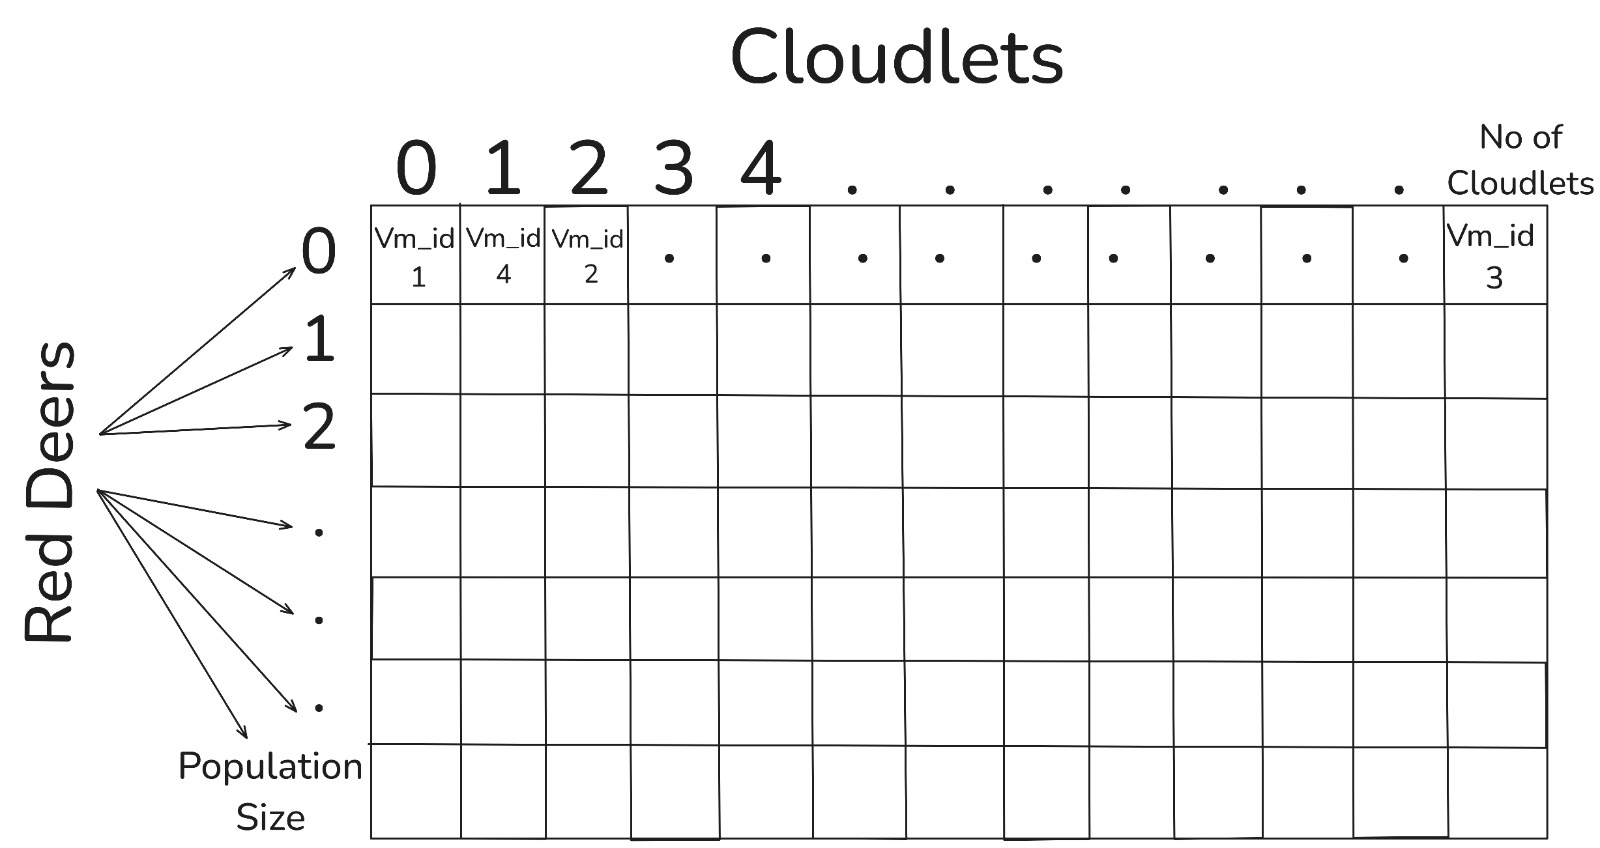
\includegraphics[width=0.9\textwidth]{Fig3.jpeg}
\caption{Mapping of each red deer with one load balancing solution}\label{Population}
\end{figure}

Once fitness values are obtained, the population is sorted in ascending order of fitness (lower is better), and the top-performing $N_{male}$(parameter which is already initially set) red deers are selected as males from which top $\gamma$\% of the males are choosen as commanders, while the remaining form the group of hinds. 

Top $N_{male}$ Red Deers are considered as males:

\begin{equation}
M = \{RD_1, RD_2, \dots, RD_{N_{\text{male}}}\}
\end{equation}

The remaining individuals are considered as hinds:

\begin{equation}
H = \{RD_{N_{\text{male}} + 1}, RD_{N_{\text{male}} + 2}, \dots, RD_{N_{\text{pop}}}\}
\end{equation}

Where Nmale shows the elitist RDs. Simply said, the number of Nmale maintains the intensification properties, while Nhind considers the diversification phase of the algorithm.

\subsection{Roaring Process}\label{subsec4.2}
In the roaring phase, each male red deer attempts to improve its current solution (i.e., cloudlet-to-VM mapping) by exploring its neighborhood in the solution space. This behavior mimics the natural tendency of red deer to expand their territory and display dominance by roaring.

\begin{figure}[h]
\centering
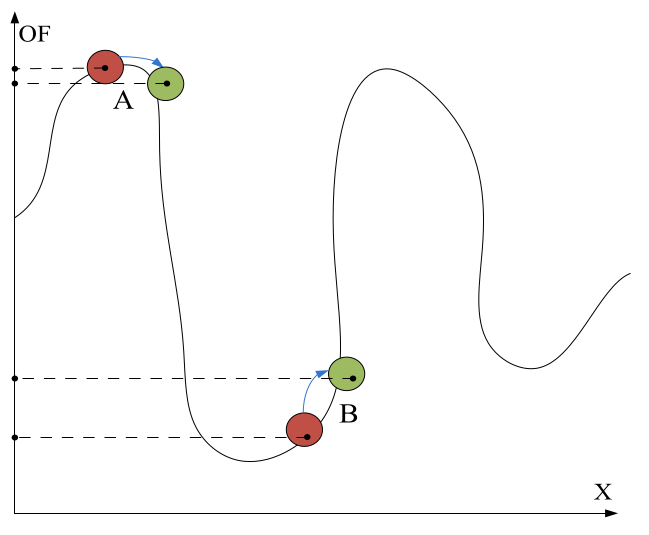
\includegraphics[width=0.9\textwidth]{Fig4.png}
\caption{Roaring Process of male red deers \cite{red_deer}}\label{Roaring}
\end{figure}

To simulate this behavior computationally, each male red deer \( RD_i \in M \) updates its position according to the following rule \cite{red_deer}:

\begin{equation}
male^{\text{new}}_i =
\begin{cases}
male^{\text{old}}_i + a_1 \cdot (((UB - LB) \cdot a_2) + LB), & \text{if } a_3 \geq 0.5 \\
male^{\text{old}}_i - a_1 \cdot (((UB - LB) \cdot a_2) + LB), & \text{if } a_3 < 0.5
\end{cases}
\end{equation}
      
Where:
\begin{itemize}
    \item \( male^{\text{old}}_i \) is the current red deer position (i.e., current cloudlet-to-VM assignment),
    \item \( male^{\text{new}}_i \) is the updated solution after roaring,
    \item \( UB = N_{VM} \) and \( LB = 0 \), which denotes the upper and lower bounds of the solution space, respectively. All the numbers in this range represent unique \texttt{vm\_id}s,
    \item \( a_1, a_2, a_3 \in [0, 1] \) are uniformly distributed random numbers.
\end{itemize}

Each male RD generates a new position using the above update rule. The updated solution is accepted only if it yields a better fitness value compared to the previous one. This ensures that the exploration during roaring leads to quality improvements in the mapping.

Figure \ref{Roaring} illustrates two scenarios chosen from the solution space to show the effect of roaring in isolation. Observe that cases A and B normally happen within the roaring period. In case A, the new position is accepted because its objective function value (eq.\ref{fitness}) is higher than that of the old position. In case B, the new solution is not acceptable. Observe again that the y-axis is the Objective function value, and the x-axis is the positions of males in this figure.

\subsection{Selection of the best male RDs as commanders}\label{subsec4.3}
In nature, not all male red deers possess the same level of strength, dominance, or attractiveness. Some exhibit superior traits and are more successful in claiming and defending territories. This variation is modeled in the RDA by classifying the male red deers into two distinct groups: \textit{commanders} and \textit{stags} \cite{red_deer}.

In our cloudlet-to-VM mapping scenario, each male RD represents a potentially optimal mapping configuration. To further intensify the search, we designate the top $\gamma$\% of male RDs (based on fitness value) as commanders, and the remaining ones as stags.

The number of commanders \( N_{\text{Com}} \) is computed using the following formula:

\begin{equation}
N_{\text{Com}} = \text{round}( \gamma \cdot N_{\text{male}} )
\end{equation}

\noindent where:
\begin{itemize}
    \item \( \gamma \in [0, 1] \) is a user-defined parameter representing the percentage of elite males to be chosen as commanders,
    \item \( N_{\text{male}} \) is the total number of male red deers.
\end{itemize}

After selecting the commanders, the remaining male RDs are assigned the role of stags. The number of stags \( N_{\text{stag}} \) is calculated as:

\begin{equation}
N_{\text{stag}} = N_{\text{male}} - N_{\text{Com}}
\end{equation}

This division of roles creates a hierarchy among the male RDs, which is later used in the fighting and mating phases \cite{red_deer}. In our implementation, we set \( \gamma = 0.4 \), meaning 40\% of male RDs are chosen as commanders which was giving experimentally best outcome.

\subsection{Fight between male commanders and stags}\label{subsec4.4}
Once the male red deers have been divided into commanders and stags, the next step is to simulate the natural behavior of dominance through fights. Each commander is randomly paired with a stag to engage in a competition to improve the population's overall fitness \cite{red_deer}. These confrontations result in the generation of new candidate solutions through exploitation of the solution space.


\begin{figure}[h]
\centering
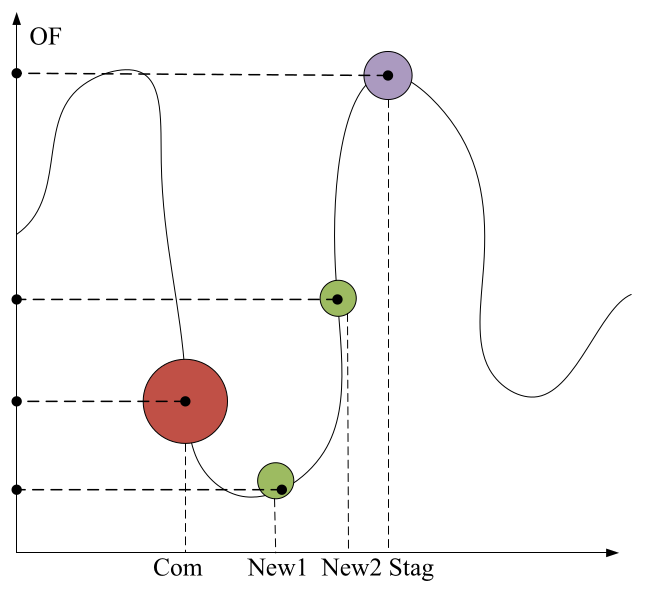
\includegraphics[width=0.9\textwidth]{Fig5.png}
\caption{Fight between a commander and a stag \cite{red_deer}}\label{Fighting}
\end{figure}

For each such pairing, two new solutions are generated using the following equations:

\begin{equation}
\text{New}_1 = \frac{(\text{Com} + \text{Stag})}{2} + b_1 \cdot ((\text{UB} - \text{LB}) \cdot b_2 + \text{LB})
\end{equation}\label{fight1}

\begin{equation}
\text{New}_2 = \frac{(\text{Com} + \text{Stag})}{2} - b_1 \cdot ((\text{UB} - \text{LB}) \cdot b_2 + \text{LB})
\end{equation}\label{fight2}

\noindent where:
\begin{itemize}
    \item \( \text{Com} \) and \( \text{Stag} \) denotes the current position vectors (solutions - Cloudlet to VMs mapping) of the commander and stag, respectively,
    \item \( b_1 \) and \( b_2 \) are random variables drawn from a uniform distribution over the interval [0, 1].
\end{itemize}

The commander is replaced with best solution after evaluating their objective function (eq.\ref{fitness}) out of all the four possible solution (commander, stag, and the two new offspring \ref{fight1}) \cite{red_deer}.

\subsection{Form harems}\label{subsec4.5}
In nature, each male commander claims a group of hinds, forming a harem based on his strength and dominance. In our solution, this behavior is simulated by associating a portion of the hinds population with each commander based on their fitness values. A lower fitness(Lower is better) implies a larger harem.

\begin{figure}[h]
\centering
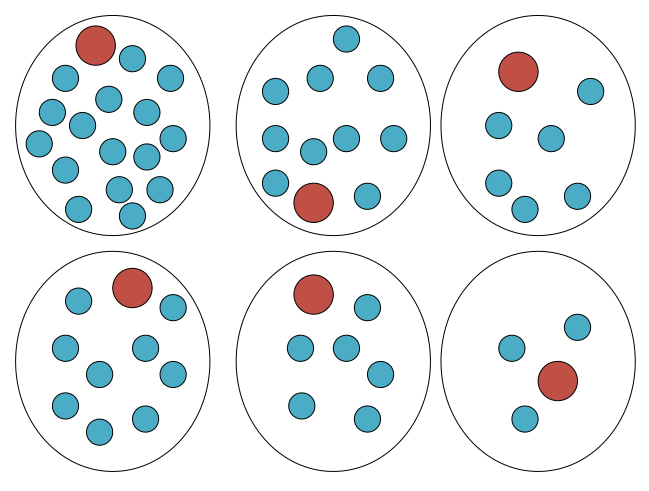
\includegraphics[width=0.9\textwidth]{Fig6.png}
\caption{Harems of each commander \cite{red_deer}}\label{Harems}
\end{figure}

Calculate the relative power \( V_n \) of each commander using the following equation:

\begin{equation}
V_n = v_n - \max\{v_i\}
\end{equation}

\noindent where:
\begin{itemize}
    \item \( v_n \) is the fitness value (objective function value) of the \( n \)-th commander,
    \item \( \max\{v_i\} \) represents the worst (here, maximum) fitness among all commanders, ensuring normalization by fitness proximity to optimality.
\end{itemize}

Then, we normalize this value to determine the portion of hinds to be assigned to each commander:

\begin{equation}
P_n = \frac{V_n}{\sum_{i=1}^{N_{Com}} V_i}
\end{equation}

\noindent where:
\begin{itemize}
    \item \( P_n \) is the normalized power of the \( n \)-th commander,
    \item \( N_{Com} \) denotes the total number of commanders.
\end{itemize}

Now, based on this proportional power, the number of hinds allocated to the \( n \)-th commander’s harem is computed as:

\begin{equation}
N.{\text{harem}_n} = \text{round}(P_n \cdot N_{\text{hind}})
\end{equation}

\noindent where:
\begin{itemize}
    \item \( N.{\text{harem}_n} \) is the number of hinds of the \( n \)-th commander's harem,
    \item \( N_{\text{hind}} \) is the total number of hinds in the population.
\end{itemize}

Hinds are then randomly assigned to commanders based on the computed values \( N.{\text{harem}_n} \). Each selected group of hinds, together with its corresponding commander, constitutes one harem.

\subsection{Mating of commanders with hinds in his harem}\label{subsec4.6}
Like other species in nature, red deer mates with each other. Here commander mates with $\alpha$\%  of hinds of his harem and generates offsprings. It is calculated as:

\begin{equation}
N.{\text{Harem}_n^{mate}} = \text{round}(\alpha \cdot N.{\text{Harem}_n})
\end{equation}

\noindent where:
\begin{itemize}
    \item $N.{\text{Harem}_n^{mate}}$ is the number of hinds from the $n$-th harem that will mate with the commander,
    \item $N.{\text{Harem}_n}$ is the total number of hinds in that harem,
    \item $\alpha$ [0-1] is a user-defined uniform model parameter that controls the mating percentage.
\end{itemize}

Once the hinds for mating are selected randomly from each harem, a new offspring (solution) is produced using the following equation:

\begin{equation}
\text{offs} = \frac{\text{Com} + \text{Hind}}{2} + c \cdot (UB - LB)
\end{equation}\label{offspring}

\noindent where:
\begin{itemize}
    \item $\text{Com}$ and $\text{Hind}$ represent the current position vectors (solutions - Cloudlet to VMs mapping) of the commander and a selected hind,
    \item $\text{offs}$ is the new offspring (i.e., the new candidate solution),
    \item $c$ is a random number generated from a uniform distribution over the interval [0, 1].
\end{itemize}


\subsection{Mating of commander with hinds of another harem}\label{subsec4.7}
Allow each commander to mate with $\beta$\% of hinds from another randomly selected harem \cite{red_deer}. 

Let $i$ be the index of a randomly selected harem which is not itself. The number of hinds in the $i$-th harem that mate with the current commander is given by:

\begin{equation}
N.{\text{Harem}_i^{mate}} = \text{round}( \beta \cdot N.{\text{Harem}_i} )
\end{equation}

\noindent where:
\begin{itemize}
    \item $N.{\text{Harem}_i^{mate}}$ is the number of hinds from the $i$-th harem that will mate with the commander,
    \item $N.{\text{Harem}_i}$ is the number of hinds in the $i$-th harem,
    \item $\beta$ is a user-defined parameter controlling the proportion of hinds involved in inter-harem mating, range value of this parameter is between zero and one.
\end{itemize}

Each of the $N.{\text{Harem}_i^{mate}}$ hinds selected from the $i$-th harem mates with the current commander using the same offspring generation formula defined in \ref{offspring}. 

\subsection{Mating of stag with the nearest hind}\label{subsec4.8}
Unlike commanders, stags do not form harems but still participate in the mating phase. Each stag mates with the hind who is nearest.

The nearest hind is determined using Euclidean distance in the $J$-dimensional solution space. The distance between a stag and the $i$-th hind is calculated as:

\begin{equation}
d_i = \sqrt{ \sum_{j=1}^{n} (\text{stag}_j - \text{hind}_{i,j})^2 }
\end{equation}

\noindent where:
\begin{itemize}
    \item $d_i$ is the distance between the stag and the $i$-th hind,
    \item $\text{stag}_j$ and $\text{hind}_{i,j}$ represent the $j$-th dimension of the stag and of the $i$-th hind, respectively,
\end{itemize}

After identifying the nearest hind (i.e., the one with the smallest $d_i$), the stag mates with it using the same equation as \ref{offspring}, replacing the commander’s role with that of the stag.


\subsection{Select the next generation}\label{subsec4.9}
The next generation is formed by combining the current solutions and newly generated offsprings. 

To achieve this, two selection strategies are used:

\begin{enumerate}
    \item \textbf{Elite Preservation:} All male red deer from the current generation, including both commanders and stags, are retained. These represent the elite solutions.
    
    \item \textbf{Offspring Selection:} The remainder of the population is filled by selecting individuals from the pool of all hinds and the offspring generated through the mating processes. This selection is performed using tournament selection method.
\end{enumerate}

\subsection{Stopping condition}\label{subsec4.10}
RDA continues its iterative process till 100 iterations which is a optimal value experimentally proven\cite{red_deer}.

Figure \ref{fig:rda-flowchart} and Alogrithm \ref{alg:rda_load_balancing} provides a summarized overview of the main steps involved in the RDA. It highlights the initialization, male classification, roaring, fighting, harem formation, mating, and selection processes that collectively guide the search for optimal load balancing in the cloud environment.


\section{Experimental Setup}\label{sec5}

Evaluating the performance of the implemented resource provisioning algorithms, including our proposed approach, in a consistent and repeatable manner across different system environments and configurations was a challenging task. To address this, we used CloudSim to simulate a virtual cloud environment. CloudSim is an open and extensible simulation framework via which cloud computing infrastructures and resource provisioning policies can be simulated and modelled. It was created at the CLOUDS Laboratory, Department of Computer and Software Engineering, University of Melbourne \cite{cloudsim}, it provides a controlled environment to conduct experiments without the need for a real cloud infrastructure. It allowed us to compare the performance of our proposed algorithm with other existing algorithms effectively. Moreover, CloudSim supports customization by enabling developers to extend or replace its core classes, making it suitable for implementing new scheduling or provisioning policies \cite{cloud-sim-ref-2}.

\begin{figure}[h]
\centering
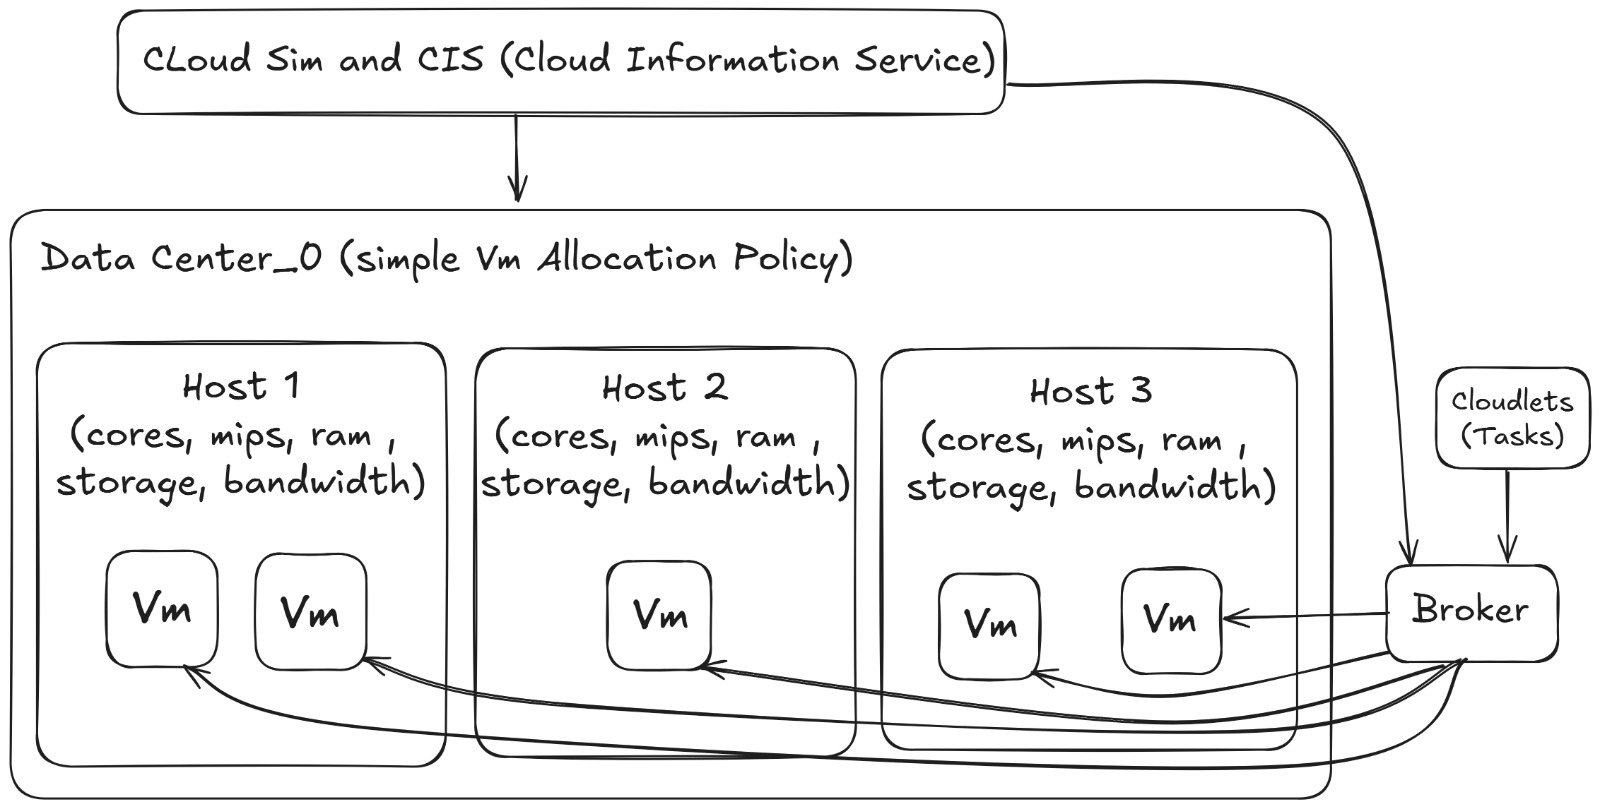
\includegraphics[width=0.9\textwidth]{Fig7.jpeg}
\caption{Basic architecture of cloudSim}\label{fig1}
\end{figure}


\subsection{Simulation data and parameters}\label{subsec2}

\begin{table}[h]
\caption{Technical Characteristics of the hosts}\label{tab1}%
\begin{tabular*}{\textwidth}{@{\extracolsep\fill}lcccccc}
\toprule
Host ID & Cores  & Processing speed, MIPS & RAM, MB 4 & Storage, MB & Bandwidth, Mbps\\
\midrule
1    & 4   & 5000  & 204,800 & 1,048,576 & 102,400 \\
2    & 2   & 2500  & 102,400 & 1,048,576 & 102,400 \\
3    & 1   & 1000  & 51,200  & 1,048,576 & 102,400 \\
\botrule
\end{tabular*}
\end{table}

\begin{table}[h]
\caption{Parameters of RDA}\label{tab2}%
\begin{tabular*}{\textwidth}{@{\extracolsep\fill}lcccccc}
\toprule
Parameters & Value \\
\midrule
Population size(no. of solutions) & 100 \\
Male population(no. of males) & 15 \\
Maximum iteration & 100 \\
Alpha(\% of hinds a commander mates with in his harem) & 0.5 \\
Beta(\% of hinds a commander mates with in another harem) & 0.2 \\
Gamma(Fraction of males selected as commanders) & 0.4 \\
LB(Lower Bound) & 0.0 \\
UB(Upper Bound) & $N_{VM}$ \\
\botrule
\end{tabular*}
\end{table}

To simulate a realistic cloud environment, we configured three hosts with varying hardware specifications, as shown in Table \ref{tab1}. These configurations were chosen to represent heterogeneous cloud resources, which is a common scenario in real-world data centers. Each host varies in terms of the number of CPU cores, processing speed (MIPS), RAM, and other attributes, allowing us to test the algorithm's performance under diverse conditions.

For RDA, the parameters listed in Table \ref{tab2} were finalized after multiple rounds of experimentation. Various combinations of population size, male-to-female ratio, and mating behavior percentages ($\alpha, \beta, \gamma$) were tested. The configuration yielding the most stable and optimal results in terms of makespan, response time, and resource utilization was selected. Specifically, a population size of 100 and 15 males with a commander selection ratio of 40\% provided a good balance between exploration and exploitation. The bounds for solution values were defined based on task and resource limits in the simulation environment.

All the experiments were performed on a Lenevo yoga 6 laptop with intel i5 $13^{th}$ generation H series processor and 16 gigabytes Ram.

\section{Results and Analysis}\label{sec6}

The RDA algorithm is especially good at reducing makespan by a synergy of smart design elements competing against one another. Combining RDA with QoS, it performs well in discovering new possibilities while optimizing current solutions. Its nature-inspired phases—roaring, fighting, and mating—stimulate diverse ideas without leaping too quickly at suboptimal solutions. The algorithm organizes its population hierarchically, separating males into commanders and stags, and hinds into harems based on their performance. This organization has the highest-performing members contributing more to future generations, leading the group towards stronger solutions. Furthermore, selective replacement keeps only the best offspring, always improving solution quality. Overall, RDA's combination of targeted fitness checks, organized population dynamics, and selective selection makes it very effective in reducing makespan.
The GWO is also successful in reducing makespan, with a leadership-based search strategy where the best solutions lead the population to promising regions. Its hierarchical organization is similar to that of a wolf pack, with alpha, beta, and delta wolves guiding the members of the sub-order towards quick convergence. GWO maintains exploration-exploitation balance through adaptive parameter adjustment at no computational cost of sophisticated genetic operators like crossover or mutation. The GWO is more probable to generate superior solution quality compared to GA since its reduced search strategy is robust while converging to high-performance configurations with improved accuracy.
This is demonstrated more clearly in Figure \ref{Makespan}.


\begin{figure}[h]
\centering
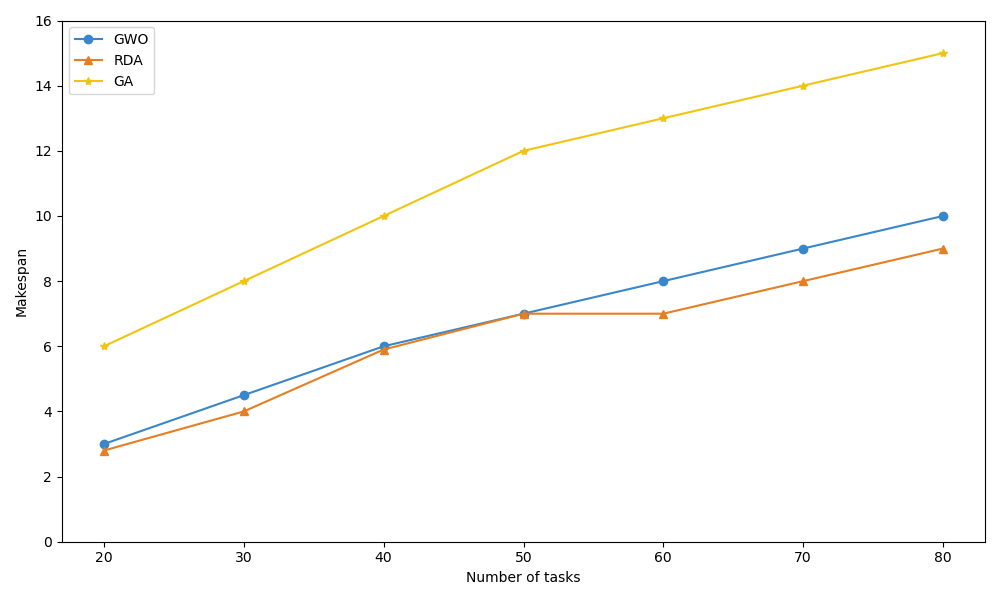
\includegraphics[width=0.9\textwidth]{Fig8.png}
\caption{Makespan Comparison}\label{Makespan}
\end{figure}

\begin{figure}[h]
\centering
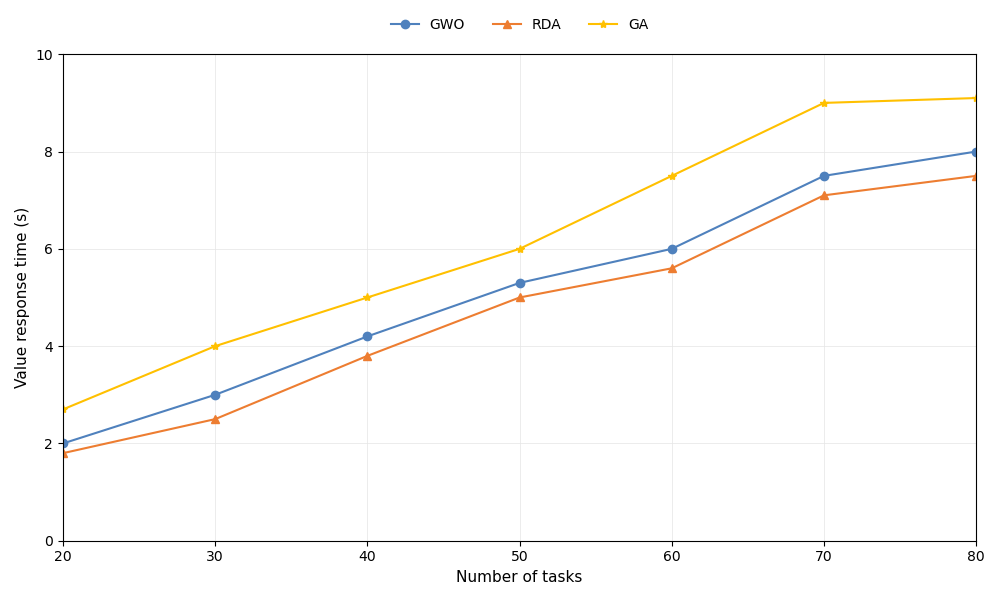
\includegraphics[width=0.9\textwidth]{Fig9.png}
\caption{Response Time Comparison}\label{Response}
\end{figure}

Figure \ref{Response} presents a detailed comparison of response times across three algorithms under evaluation, with task counts configured at 20, 30, 40, 50, 60, 70, and 80. Response time, a critical metric to minimize, is calculated by aggregating the execution durations of individual services to determine the total time required for composite function processing. The results, as depicted in the figure, underscore the superior efficiency of the proposed algorithm in optimizing response time.

\begin{figure}[h]
\centering
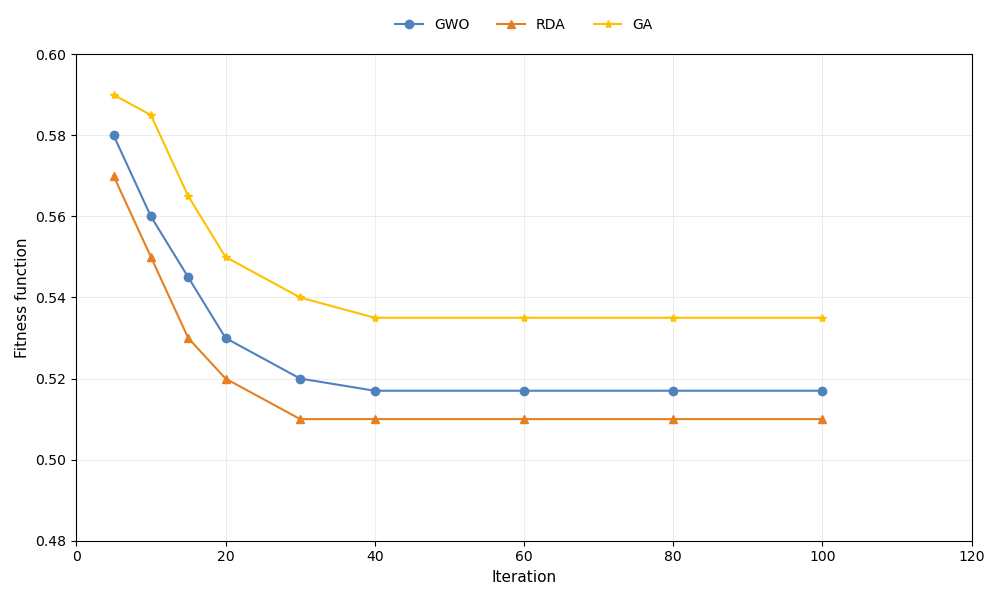
\includegraphics[width=0.9\textwidth]{Fig10.png}
\caption{Convergence Comparison}\label{Convergence}
\end{figure}

To evaluate the convergence behavior of the RDA, it was pitted against GA and GWO over 100 iterations. As illustrated in Figure \ref{Convergence}, the convergence test involved 80 tasks, across 100 iterations, highlighting how the algorithms stack up in terms of solution refinement.

The RDA offers a highly effective approach to load balancing in distributed, grid, and cloud computing environments, offering distinct advantages over traditional approaches through its optimization framework. By modeling the complex mating rituals of red deer—particularly their roaring competitions, territorial conflicts, and harem establishment processes—RDA effectively navigates the crucial balance between exploration and exploitation phases that often challenge other algorithms. When used in cloud resource allocation, RDA is very effective in the way that it considers both existing system loads and QoS demands simultaneously, thus avoiding resource saturation and underutilization.
Our work confirms that RDA consistently outperforms rival evolutionary algorithms such as the GWO and GA, particularly at high loads. The strongest aspect of the algorithm is its ability to dynamically adapt based on evolving conditions. Our simulation evidence in real data attests to the improved performance of RDA on vital parameters such as reduced makespan and enhanced response time, although rival algorithms occasionally display increased fitness values in specific constraint cases.
The combination of quality-driven resource allocation with principles of biologically-inspired optimization allows RDA to solve the complicated issues inherent in current cloud computing. The integration offers a solution that, apart from optimizing task execution efficiency, balances the system irrespective of the loading status. Such results indicate that RDA offers an incredibly practical way of solving computing systems for which timely provision of services and balancing workloads are critical operational needs.



\section{Conclusion and Future Work}\label{sec7}

This study evaluates the RDA for cloud load balancing, demonstrating that this nature-inspired method effectively addresses resource allocation challenges and outperforms conventional and other metaheuristic algorithms like GWO and GA in reducing makespan time, and response times and in increasing cost efficiency, and resource utilization primarily due to its balanced exploration and exploitation capabilities; furthermore the algorithm presents avenues for enhancement through integration with machine learning and multi-criteria decision making, along with evaluations of expanded systems and additional QoS factors to bolster real-world cloud adaptability.
In the future, studies can explore whether RDA can be used together with other smart algorithms or methods. It can also examine its performance on extremely large data sets and compare its performance with deep learning algorithms to determine how they can complement each other. Future studies can also explore how the fitness function can be enhanced by incorporating other elements such as Jain's fairness Index \cite{Jain_fairness_index} and exploring how stable the algorithm's reliability is and how stable the quality of the service is.



%%===========================================================================================%%
%% If you are submitting to one of the Nature Portfolio journals, using the eJP submission   %%
%% system, please include the references within the manuscript file itself. You may do this  %%
%% by copying the reference list from your .bbl file, paste it into the main manuscript .tex %%
%% file, and delete the associated \verb+\bibliography+ commands.                            %%
%%===========================================================================================%%

\bibliography{sn-bibliography}
% common bib file
%% if required, the content of .bbl file can be included here once bbl is generated
%%\input sn-article.bbl


\end{document}
